\begin{figure}[t]
\centering
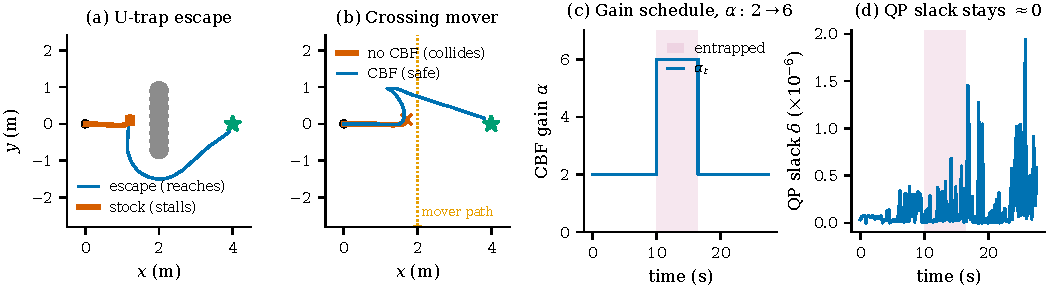
\includegraphics[width=\linewidth]{figures/mechanism.pdf}
\caption{\textbf{Mechanism validation in the 2D mirror} (seed-fixed single runs; \cref{tab:mechanism}). \textbf{(a)}~Stock MPPI stalls at the mouth of a finite wall ($x\approx1.2$\,m) while the detection-and-escape layer rounds it to the goal. \textbf{(b)}~Against a mover crossing the path, the no-CBF controller collides ($\times$) while the look-ahead-point CBF filter keeps the robot clear. \textbf{(c,\,d)}~On the U-trap, the coordinated gain rises from $\alpha_{\mathrm{base}}{=}2$ to $\alpha_{\mathrm{escape}}{=}6$ while entrapped (shaded) and the QP slack stays below $2\times10^{-6}$ throughout: the escape is admitted without relaxing the barrier, close to the slack-free setting that \cref{prop:invariance} assumes. Regenerated as vector graphics by \texttt{scripts/make\_figures.py}.}
\label{fig:mechanism}
\end{figure}
